En este capítulo se explica el porqué se han tomado ciertas decisiones, problemas y dudas que han ido surgiendo a lo largo del desarrollo y se muestra las especificaciones del sistema.

\section{Consideraciones de Diseño}
Cuando se utiliza GitHub en el ámbito académico no hay una sola forma de organizar las clases y queda a criterio de cada profesor. Es por esto que una aplicación inflexible no puede llegar muy lejos. Como resultado, se ha decidido crear una sistema generalista en el que permita al usuario modificar lo máximo posible el resultado final. Todo esto se puede realizar gracias a un archivo de configuración, el cual permite tanto modificar la apariencia de la aplicación como el propio contenido de esta.

El hecho de que ciertos apartados de la aplicación no estén en el ecosistema de GitHub llega a ser un gran problema, ya que no se pueden obtener por la API de GitHub, por esto se permite que los enlaces a esas secciones se puedan introducir a través de la configuración. Por lo que se permitirá cambiar cosas como el nombre de la aplicación y los enlaces a los diferentes contenidos como el google classroom o parecidos, campus virtual de la asignatura, etc.

Otro punto a destacar sería el hecho de que muchas veces un profesor puede querer relacionar ciertos contenidos como las clases, labs o temas entre ellos. Es por esto que para simplificar la experiencia del usuario se les permite introducir en el encabezado de los diferentes archivos markdown, las key de otros archivos para poner enlaces a ellos de manera automática en la página creada.

\section{El inicializador de {\tt adastra}}
Como punto de inicio para usar la aplicación se ha decidido seguir un patrón que siguen la gran mayoría de paquetes en el ámbito de desarrollo de aplicaciones con Javascript y npm. Este se basa en usar el comando \verb|create| de los manejadores de paquetes como npm o yarn. El comando de inicio de adastra sería el siguiente:

\begin{verbatim} pnpm create adastra-lms\end{verbatim}
Este comando buscará un paquete con el nombre \verb|create-{name}|, siendo el \verb|name| el parámetro que se le pase al comando, en este caso para adastra sería el paquete \verb|create-adastra-lms| y se ejecutaría para crear un proyecto la aplicación. Este sistema lo usan la mayoría de framework populares de JS como React o incluso Astro, el framework usado por esta aplicación.

\section{La template del proyecto}
Tras haber ejecutado el comando anterior se creará el proyecto en función de la template que se ha creado para este. Dentro de esta se ha dotado de muchas funcionalidades para simplificar y mejorar la experiencia del usuario.

\subsection{Creación de contenido por Markdown}
El sistema más fundamental sería la creación del contenido principal de la aplicación que en este caso se divide en tres carpetas (labs, classes y subjects), en las cuales se podrá añadir nuevos archivos de tipo markdown con el fin de añadir contenido al LMS.

En este caso el contenido de cada carpeta está pensado para que se use de la siguiente manera:
\begin{itemize}
    \item \textbf{labs}: Comprendería las tareas y laboratorios de la asignatura.
    \item \textbf{classes}: Aquí irían información sobre las clases impartidas. Normalmente separando el contenido en días.
    \item \textbf{subjects}: Por último serían la información relacionadas con los diferentes temaríos de la asignatura. Normalmente habrá una o más clases y labs relacionadas con un subject.
\end{itemize}

\subsection{El sistema de navegación en función de la rutas}
Uno de los sistemas que más fácilmente se puede ver es que a lo largo del proyecto es que a la izquierda de la web producida se encontraría una barra de navegación que de forma automática. Este sistema se divide en tres partes \verb|tabs|(pestañas), \verb|sections|(secciones) y \verb|entries|(entradas). De base la aplicación está diseñada para que tenga dos \verb|tabs|, en la que cada una tiene múltiples \verb|sections| con uno o más \verb|entries| por cada una. En la figura \ref{fig:navigationSystem} se pueden ver como quedarían las diferente partes del sistema de navegación en el diseño final.

\begin{figure}
    \centering
    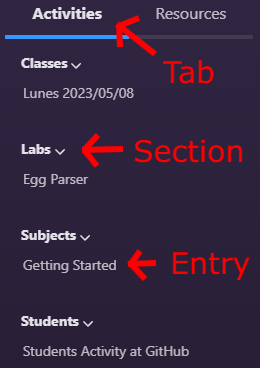
\includegraphics{images/navigationSystem.png}
    \caption{Barra lateral con las diferentes partes del sistema de navegación}
    \label{fig:navigationSystem}
\end{figure}

Con esto nos encontramos con un problema y es que de base como se crean las páginas en función de la ruta que tenga, terminaría por ordenar cada parte de la navegación alfabéticamente. Esto le quita flexibilidad a la aplicación, por lo que se decide que el usuario deberá añadir en cada parte de la ruta del archivo un número que simboliza el orden que deba tener usando \verb|-| como separador. Es decir unas rutas como las siguientes:

\begin{verbatim}
    virtual/class/prueba.md
    virtual/class/test.md
\end{verbatim}

Tendrían un orden alfabético pero al añadir los números para así ordenar quedarían como los siguientes:

\begin{verbatim}
    1-virtual/1-class/1-test.md
    1-virtual/1-class/2-prueba.md
\end{verbatim}


\subsection{El fichero de Configuración {\tt adastra.config.mjs}} \label{diseño:data}
Uno de los puntos claves al crear está template fue buscar la mayor flexibilidad posible a la hora de poder modificar los contenidos por el usuario, pero sin complicar demasiado el proceso. Es por eso que en un punto se decidió crear un archivo de configuración en que poder especificar ciertos cambios sin tener que modificar el código directamente el usuario.

Dentro de este archivo se estableció dos posibles configuraciones que el usuario quería cambiar:
\begin{itemize}
    \item \textbf{tailwindConfig}: En esta sección se podrá añadir cambios a la propia configuración de la librería de estilos usada por la template para así poder modificar la apariencia de la aplicación de manera sencilla.
    \item \textbf{organizationInfo}: La última sección, pero no menos importante, serviría para añadir nueva información que la aplicación no pueda obtener de la API de GitHub o que se quiera que el usuario pueda decidir que añadir. Algunos ejemplos de esto sería el título que saldría en la aplicación o el link a el campus virtual de la asignatura.
\end{itemize}

En la figura \ref{fig:adastraConfig} se puede ver un ejemplo de la configuración.